% figure: 现控强化1-23-精确观测器结构图.png
\documentclass[border=10pt]{standalone}
\usepackage{fontspec}
\setmainfont{Cambria}
\usepackage{unicode-math}
\setmathfont{Cambria Math}
\usepackage{tikz}
\usetikzlibrary{arrows.meta,calc}
\begin{document}
\begin{tikzpicture}[>=Stealth,line width=.9pt,
 b/.style={draw,minimum width=1.2cm,minimum height=.75cm,fill=blue!4},
 s/.style={draw,circle,minimum size=.45cm,inner sep=0pt}]
\node[b] (b) at (0,0) {$B$};
\node[s] (s) at (2,0) {$+$};
\node[b] (i) at (4,0) {$\dfrac{E_3}{s}$};
\node[b] (c) at (7,0) {$C$};
\node[s] (err) at (9,-2) {$+$};
\node[b] (h) at (5,-2) {$h$};
\node[b] (a) at (4,1.7) {$A$};
\draw[->] (-2,0) -- node[above] {$u\in\mathbb R^2$} (b);
\draw[->] (b) -- (s);
\draw[->] (s) -- node[above] {$\dot{\hat x}$} (i);
\draw[->] (i) -- node[below] {$\hat x\in\mathbb R^3$} (c);
\draw[->] (c) -| (err.north);
\node at (8.65,-1.65) {$-$};
\node at (9.38,-1.68) {$+$};
\draw[->] (11,-2) -- node[above] {$y$} (err);
\draw[->] (err) -- node[below] {$y-C\hat x$} (h);
\draw[->] (h) -| (s.south);
\fill (5.5,0) circle (1.5pt);
\draw[->] (5.5,0) |- (a.east);
\draw[->] (a.west) -| (s.north);
\node[anchor=north] at (4.5,-3) {$a=0.57,\quad b=0.22,\quad c=1.3$};
\node[anchor=north] at (4.5,-3.65) {$h=\begin{bmatrix}5+a(b^2+c^2)\\1+b^2+c^2+2ab\\a+2b-3\end{bmatrix}$};
\node[anchor=north] at (4.5,-5.4) {$\dot{\hat x}=A\hat x+Bu+h(y-C\hat x)$};
\end{tikzpicture}
\end{document}
